\section{Evaluation}
\label{sec:evaluation}

Our evaluation tests two claims: AutoTerm-SST eliminates pre-session setup
without sacrificing terminology accuracy or translation quality, and its fixed
working-set budget avoids the degradation of large merged glossaries.

\begin{figure*}[t]
  \centering
  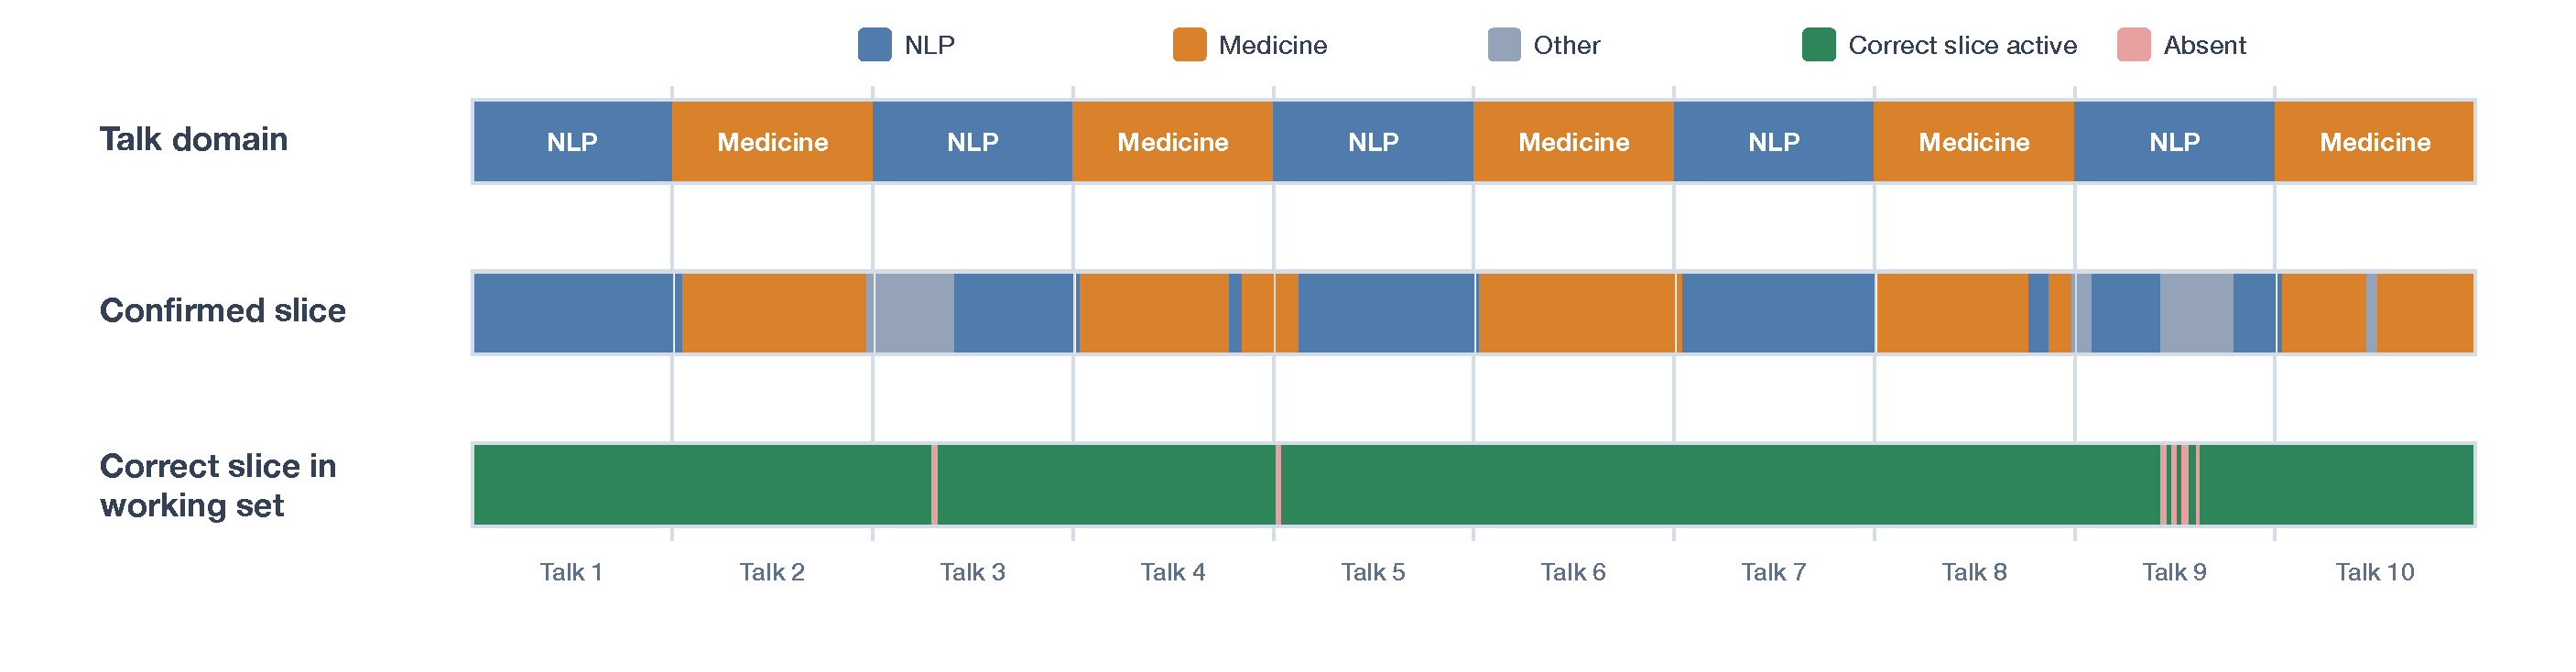
\includegraphics[width=0.96\textwidth]{routing_timeline_10talk.pdf}
  \caption{Routing trajectory of AutoTerm-SST across the ten alternating talks
  of run 1. The confirmed slice can lag briefly after topic boundaries, yet the
  four-slice working set keeps the correct glossary searchable in 96.9\% of
  decoding windows. Talk widths are normalized for readability.}
  \label{fig:routing}
\end{figure*}

\subsection{Experimental setting}

\paragraph{Data.}
We build one continuous 4.7-hour English-to-Chinese stream by alternating five
English ACL 60/60 dev talks with human-annotated
terminology~\citep{salesky-etal-2023-evaluating} and five long-form oncology
lectures from the European School of Oncology, or ESO, test
set~\citep{iranzosanchez2025eso}. Following RASST~\citep{luo2026rasst}, we
evaluate ESO with its model-generated Chinese references and manually verified
ESO terminology. Because the NLP and medicine slices hold the benchmark
glossaries, this stream measures how reliably routing keeps target terms
competitive under a fixed budget.

\paragraph{Baselines.}
All policies share RASST's model, chunks, retriever, threshold, candidate
slots, and prompt cap, and differ only in which entries are searchable.
InfiniSST~\citep{ouyang2025infinisst} runs the same streaming model without
retrieval. Known-domain-1k searches only the 1,000-entry slice matching the
current talk's domain and therefore requires the domain label of every talk.
AutoTerm-SST routes over ten 1,000-entry slices spanning NLP, medicine, and
eight topics drawn from Wikipedia and Wikidata, with at most four active at
once. Merged-2k pools the NLP and medicine slices, which still requires knowing
both domains of the stream. Merged-10k pools all ten slices into 9,880 entries
after removing exact duplicates. Merged-100k and Merged-1M expand the same NLP
and medicine glossaries with entries from other topics, and Merged-100k
consists of the first 100,000 entries of Merged-1M. All merged glossaries
retain conflicting translations of shared source terms.

\paragraph{Runs.}
Run 1 evaluates InfiniSST, Known-domain-1k, AutoTerm-SST, Merged-100k, and
Merged-1M on one H200 GPU. Run 2 repeats Known-domain-1k and AutoTerm-SST on
two A6000 GPUs and adds Merged-2k and Merged-10k. Within a run, all policies
see the same audio order and chunk boundaries.

\paragraph{Metrics.}
Following RASST, terminology accuracy, or TERM\_ACC, is the share of 2,047 time-aligned
term occurrences, 1,368 NLP and 679 medicine, whose reference translation
appears in the aligned hypothesis. For translation quality,
mWERSegmenter~\citep{matusov-etal-2005-evaluating} first resegments each talk
to the reference boundaries of the StreamLAAL
protocol~\citep{papi2024streamatt}, and we then compute corpus
SacreBLEU~\citep{papineni-etal-2002-bleu,post-2018-call}. Masked-term BLEU, or
MT-BLEU, repeats this scoring after masking every evaluated target term in both
hypothesis and reference to measure the translation around the terms. Prompt
precision is the share of injected term pairs matching a gold term in the
surrounding audio. To compare two policies, an exact permutation test swaps
their outputs talk by talk over all $2^{10}$ combinations, and a talk-level
bootstrap stratified by corpus yields 95\% confidence intervals. We write
symmetric intervals as $a\pm h$ and asymmetric intervals spanning $a-l$ to
$a+u$ as $a^{+u}_{-l}$; Appendix~\ref{app:stats} reports every paired
comparison.

\subsection{Results}

\paragraph{Comparison with the known-domain reference.}
AutoTerm-SST performs on par with a known-domain reference without receiving
any user input. In run 1, AutoTerm-SST differs from Known-domain-1k by
$+0.2\pm1.2$ TERM\_ACC points at $p=0.86$ and by $-0.10^{+0.48}_{-0.40}$ BLEU
at $p=0.70$. Run 2 on separate GPUs again shows no significant difference, as
Table~\ref{tab:stats} reports. Both retrieval-augmented policies exceed
retrieval-free InfiniSST by about 27 TERM\_ACC points, as
Table~\ref{tab:quality} shows.

\paragraph{Effect of catalog scale.}
Merged glossaries keep pace with AutoTerm-SST up to 10k entries, yet lose
translation quality and terminology accuracy as the catalog grows further. In
run 2, Merged-2k and Merged-10k remain within 0.8 TERM\_ACC points of
AutoTerm-SST with matching BLEU, and the largest gap, to Merged-10k, has
$p=0.08$. In run 1, Merged-100k maintains TERM\_ACC but loses
$1.37^{+0.43}_{-0.51}$ BLEU at $p=0.004$. Scaling to Merged-1M widens the
deficit to $3.9\pm1.9$ TERM\_ACC points at $p=0.012$ and
$2.30^{+0.65}_{-0.59}$ BLEU at $p=0.002$, concentrated on medicine with a
7.4-point loss against 2.2 points on NLP. AutoTerm-SST caps per-chunk search at
4k entries, a budget that adding slices to the catalog does not change.

\paragraph{Effect of prompt noise.}
Large merged glossaries fill the fixed prompt with irrelevant pairs, which also
lowers the quality of the surrounding translation. As Table~\ref{tab:quality}
shows, Merged-1M injects nine times as many pairs per chunk as AutoTerm-SST at
one tenth of its prompt precision. On the 935 of 1,905 sentences whose
references contain no glossary term, AutoTerm-SST still leads Merged-1M by
2.19 BLEU at $p=0.023$.

\paragraph{Routing behavior.}
Pinning the confirmed slice inside a four-slice working set shields terminology
coverage from transient ranking errors. In run 1, the confirmed slice alone is
correct in 88.5\% of decoding windows, whereas the four-slice working set keeps
the correct glossary searchable across nearly the entire stream, as
Figure~\ref{fig:routing} shows. Pinning accounts for most of this gain: without
pinning, the four highest-scoring slices by raw similarity cover only 85.0\% of
windows. Open-loop replays in Appendix~\ref{app:router} show that the router
also tracks switches between NLP and medicine every 15 to 300 seconds. Routing
still lags at abrupt talk boundaries, where stale context briefly kept the
medicine slice out of the working set after one ACL-to-medicine switch.

\paragraph{Latency and speed.}
The full pipeline keeps pace with live speech. In a single session on two
A6000 GPUs, the first translation appears 2.3 seconds after audio starts, and
each chunk returns its text 0.57 seconds after it is sent at the median and
1.17 seconds at the 95th percentile. On one H200 GPU, AutoTerm-SST processes
the stream at a real-time factor of 0.406, the processing time divided by the
audio duration, within 0.02 of Known-domain-1k; routing and retrieval average
203 milliseconds per chunk.
